\PID
Функција преноса континуалног система дата је изразом $H(s) = \dfrac{K_0}{\uptau^{-1} + s}$, где су $K_0 = 2$ и $\uptau = 0,5\unit{s}$. 
За симулацију овог система на дигиталном рачунару оваквог, потребно је овакав континуални модел дискретизовати. 
Један од начина да се то уради јесте да се одредити импулсни одзив $h(t)$, па да се на основу њега одреди 
дискретизовани импулсни одзив $\hat h[n] = T_{\rm s} \, h(nT_{\rm s})$, где је $T_{\rm s}$ периода дискретизације. 
На основу дискретизованог импулсног одзива одреди се дискретан модел $\hat H(z) = \ZT{\hat h[n]}$. 
\begin{enumerate}[label=(\alph*)]
    \item Одредити импулсни одзив $h(t)$ и његов дискретизовани еквивалент $\hat h[n]$.
    \item Одредити функцију преноса дискретизованог система $\hat H(z)$. 
    \item Одредити одзив $f(t)$ континуалног система $H(s)$ на континуалну побуду $\uu(t)$. 
    \item Одредити одзив $\hat f[n]$ дискретизованог система $H(z)$ на еквивалентну дискретну побуду $\uu[n]$. 
    \item Посматрајући континуални одзив из тачке (в) и дискретни одзив из тачке (г), упоредити их у одговарајућим тренуцима, одређивањем
          њихове разлике $\upepsilon[n] = f(nT_{\rm s}) - \hat f[n]$, која заправо представља меру грешке дискретизованог модела. 
          Одредити грешку овакве дискретизације $\upepsilon[\infty]$ у случају када је $T_{\rm s} \ll \uptau$.
\end{enumerate}

\RESENJE
(а) Полазећи од дате функције преноса континуалног система таблично, на основу \reft{T:LT:exp} се одређује његов импулсни одзив као 
\begin{eqnarray}
    h(t) = \ILT{H(s)} = K_0 \ee^{-t/\uptau} \uu(t).
\end{eqnarray}

(б) Према описаном поступку, дискретизована верзија овог сигнала добија се као 
\begin{eqnarray}
    \hat h[n] = T_{\rm s} h(nT_{\rm s}) 
    = K_0 T_{\rm s} \ee^{-nT_{\rm s}/\uptau} \uu(nT_{\rm s}) 
    = K_0 T_{\rm s} a^n \uu[n] \quad \text{, где је }\quad a = \ee^{-T{\rm s}/\uptau}
\end{eqnarray}
Користећи таблични резултат \reft{T:z:exp} добија се дискретан еквивалент 
\begin{eqnarray}
    \hat H(z) = K_0 T_{\rm s}  \dfrac{z}{z - a}
\end{eqnarray}

(в) Одскочни одзив континуалног система налазимо помоћу инверзне Лапласове трансформације као 
\begin{eqnarray}
    f(t) = \ILT{\dfrac{H(s)}{s}} = \ILT{ \dfrac{K_0}{s(s+\uptau^{-1})} } 
         = K_0 \uptau (1 - \ee^{-t/\uptau}) \uu(t)
\end{eqnarray}
%
\begin{figure}[b!]
    \centering
    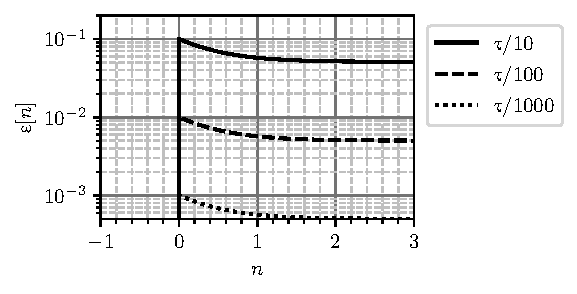
\includegraphics{fig/disk_error.pdf}
    \caption{Грешка дискретизације за различите $T_{\rm s}$.}
\end{figure}
%
(г) Oдскочни одзив дискретизованог система налази помоћу инверзне $\mathcal{Z}$-трансформације
\begin{eqnarray}
    \hat f[n] = \IZT{ \dfrac{z}{z-1} \cdot \hat H(z) } = K_0 T_{\rm s} \IZT{ \dfrac{z^2}{(z-1)(z-a)} }
    = K_0 T_{\rm s} \dfrac{1 - a^{n+1}}{1 - a} \uu[n]
\end{eqnarray}
(д) Континуалан сигнал у дискретним тренуцима $t = nT_{\rm s}$ има вредности 
\begin{eqnarray}
    f(nT_{\rm s})
    =K_0 \uptau (1 - \ee^{-nT_{\rm s}/\uptau}) \uu(t)
    =K_0 \uptau (1 - a^n) \uu[n],
\end{eqnarray}
па је онда 
\begin{eqnarray}
    \upepsilon[n] = f(nT_{\rm s}) - \hat f[n] = 
    \left( K_0 \uptau (1 - a^n) - K_0 T_{\rm s} \dfrac{1 - a^{n+1}}{1 - a} \right) \uu[n]
\end{eqnarray}


Заменом конкретних вредности $T_{\rm s} \in \left\{ 
    \dfrac{\uptau}{10}, 
    \dfrac{\uptau}{100},
    \dfrac{\uptau}{1000}
\right\}$ 
Када $n$ постаје велико тада је 
\begin{eqnarray}
    \upepsilon[\infty] &=& K_0 \left( \uptau (1 - \cancelto{0}{a^{\infty}}) + \dfrac{T_{\rm s}}{1 - a}(1 - \cancelto{0}{a^{\infty + 1}}\,\,\,\,\,) \right)
    = K_0 \left( \uptau + \dfrac{T_{\rm s}}{1 - a}  \right) \label{eq:\ID.1}
\end{eqnarray}
У случају када је $T_{\rm s}/\uptau \ll 1$ параметар $a$ се може апроксимирати линеарним чланом Тејлоровог 
реда\footnote{Користи се апроксимација $\ee^x \approx 1 + x$, за $x \ll 1$.} у облику 
$а = \ee^{-T_{\rm s}/\uptau} \approx 1 + T_{\rm s}/\uptau$, па се заменом у \ref{eq:\ID.1} има резултат
\begin{eqnarray}
    \upepsilon[\infty] &=& 
    K_0 \left( \uptau + \dfrac{\cancel{T_{\rm s}}}{-\cancel{T_{\rm s}}/\uptau}  \right)
    = K_0(\uptau - \uptau) = 0.
\end{eqnarray}

На овај начин је показано да се смањивањем периода дискретизације могу ублажити ефекти који су описани у овом задатку. 
На овој идеји се темељи низ различитих метода дискретизације континуалних система, а уопштењем поступка се добија тзв. 
\textit{импулсно-инваријантна трансформација}. На сличан начин, дискретизацијом одскочног одзива изводи се 
тзв. \textit{степ-инваријантна трансформација}. Овакве теме имају значајно место код система дигиталног управљања где је потребно добити 
дигитални модел управљаног система који је у природи континуалан. 
